\section{Results}
In this section, results from silulations made with the final version of the software are presented. Plots are included when it has been considered as important to show how a property has developed during the simulations. The simulation setups are explained in the Simulations section of this report. For an analys and discussion of the result, se Analysis section.
\subsection{Bulk averages}

Following average values were obtained for the bulk simulation:
\begin{itemize}
	\item Kinetic energy: 258.17 eV
	\item Potential energy: -9886.78 eV
	\item Total energy: -9628.99 eV
	\item Cohesive energy: -2.41 eV
	\item MSD: 0.0395 Å
	\item Internal Pressure: 3.61*10\textsuperscript{8} Pa
	\item Temperature: 499.329 K
	\item Debye temperature: 329.375 K
	\item Specific heat: 173.46 J/kg K
	\item Diffusion coefficient: 0.012 Å\textsuperscript{2}/fs
\end{itemize}

\subsection{Surface averages}
Following average values were obtained for the surface simulation:
\begin{itemize}
	\item Kinetic energy: 51.68 eV
	\item Potential energy: -1597.38 eV
	\item Total energy: -1545.7 eV
	\item Cohesive energy: -1.93 eV
	\item MSD: 0.40 Å
	\item Internal Pressure: 1.01*10\textsuperscript{9} Pa
	\item Temperature: 499.78 K
	\item Debye temperature: 102.39 K
	\item Specific heat: 173.46 J/kg K
	\item Diffusion coefficient: 8.86*10\textsuperscript{-18} Å\textsuperscript{2}/fs
\end{itemize}

\subsection{Plots}
\subsubsection{Total energy (bulk)}
The total showed a fluctruation of at most 0.1\% of the average value. The value of the total energy is equal to the sum of the potantial and the kinetic energy (see figure  \ref{totale}).
\begin{figure}[h]
	\centering
	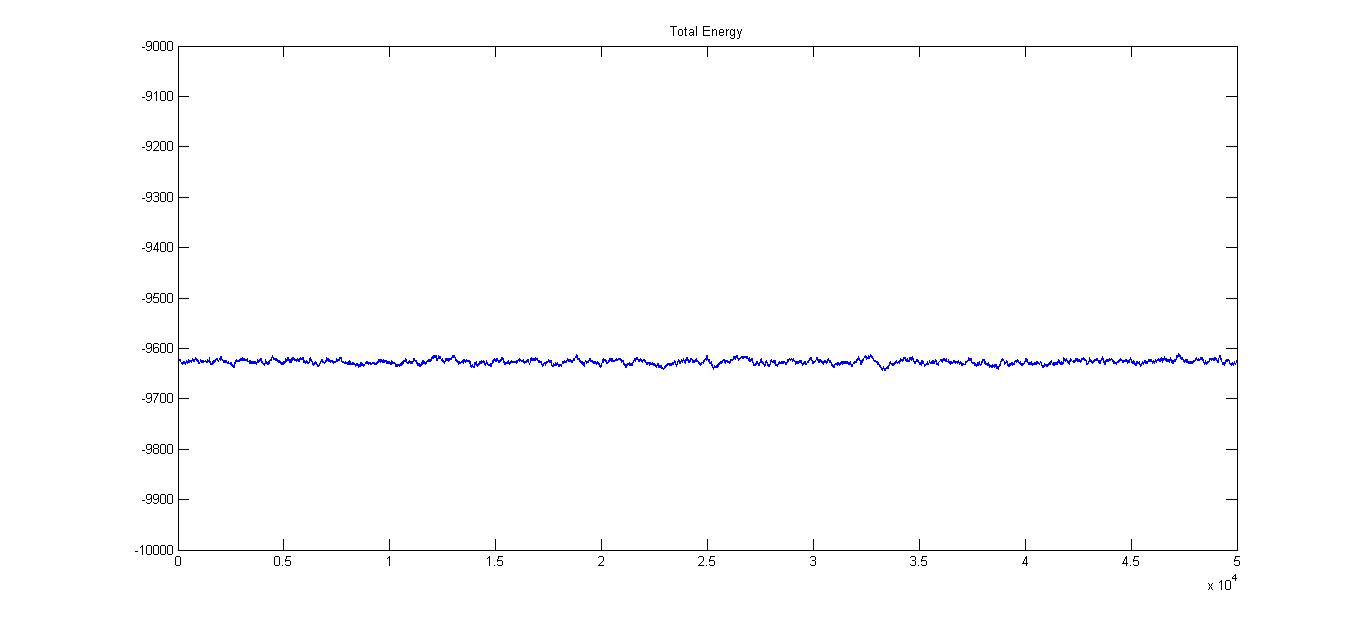
\includegraphics[width=0.7\textwidth]{total1.jpg}
	\caption{Plotted values of the total energy for bulk simulation over 50000 timesteps.}
	\label{totale}
\end{figure}

\subsubsection{Kinetic energy (bulk)}
After reaching equilibrium, the kinetic energy had a maximum fluctruation of 5\% from the average value (see figure \ref{kinetic}).
\begin{figure}[H]
	\centering
	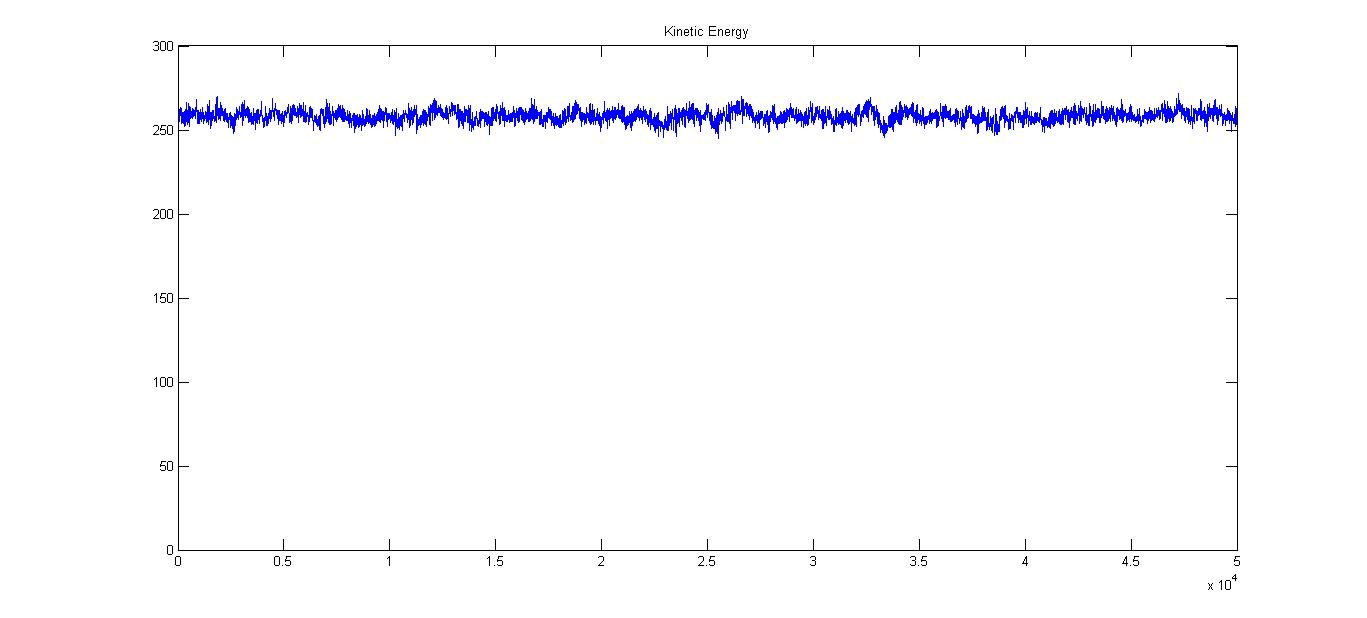
\includegraphics[width=0.7\textwidth]{kinetic.jpg}
	\caption{Plotted values of the kinetic energy for bulk simulation over 50000 timesteps.}
	\label{kinetic}
\end{figure}

\subsubsection{Kinetic energy (surface)}
See figure \ref{kineticsf}.
\begin{figure}[h]
	\centering
	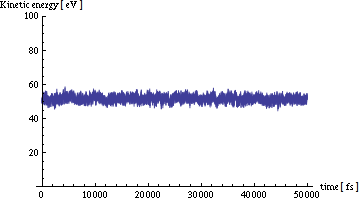
\includegraphics[width=0.7\textwidth]{kinetic_surface.png}
	\caption{Plotted values of the kinetic energy for ssurface simulation over 50000 timesteps.}
	\label{kineticsf}
\end{figure}

\subsubsection{Diffusion coefficient (bulk)}
See figure \ref{diff}.
\begin{figure}[h]
	\centering
	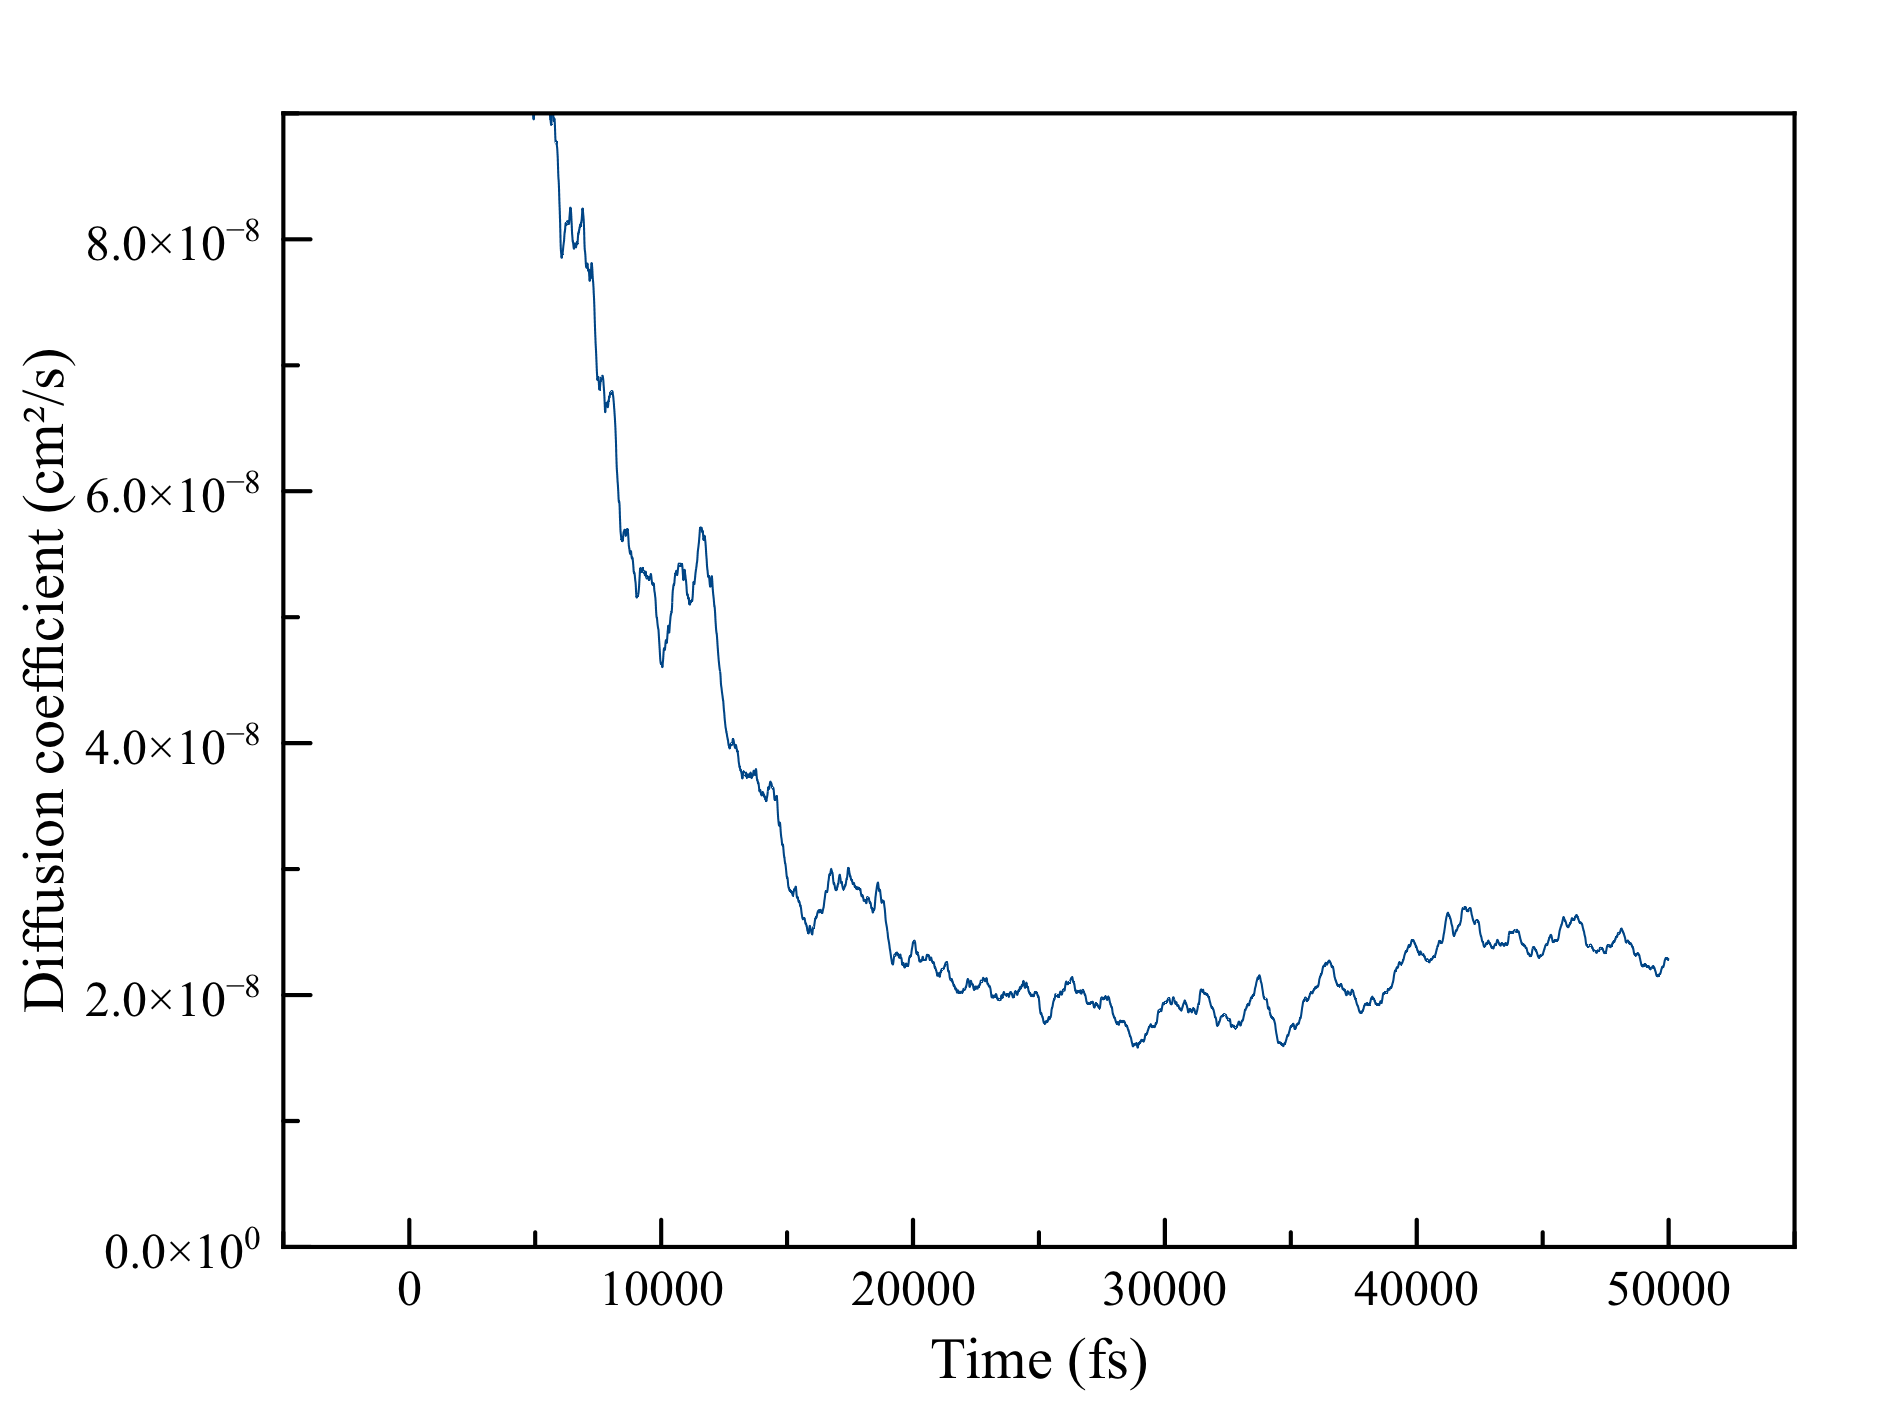
\includegraphics[width=0.7\textwidth]{Diffusion_coeff.png}
	\caption{Plotted values of the diffusion coefficient for bulk simulation over 50000 timesteps.}
	\label{diff}
\end{figure}

\subsubsection{Diffusion coefficient (surface)}
See figure \ref{diffsf}.
\begin{figure}[H]
	\centering
	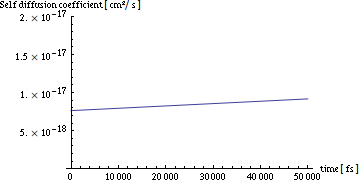
\includegraphics[width=0.7\textwidth]{diffusion_coeff_surface.png}
	\caption{Plotted values of the diffusion coefficient for surface simulation over 50000 timesteps.}
	\label{diffsf}
\end{figure}


\subsubsection{Debye Temperature (bulk)}
See figure \ref{debye}.
\begin{figure}[H]
	\centering
	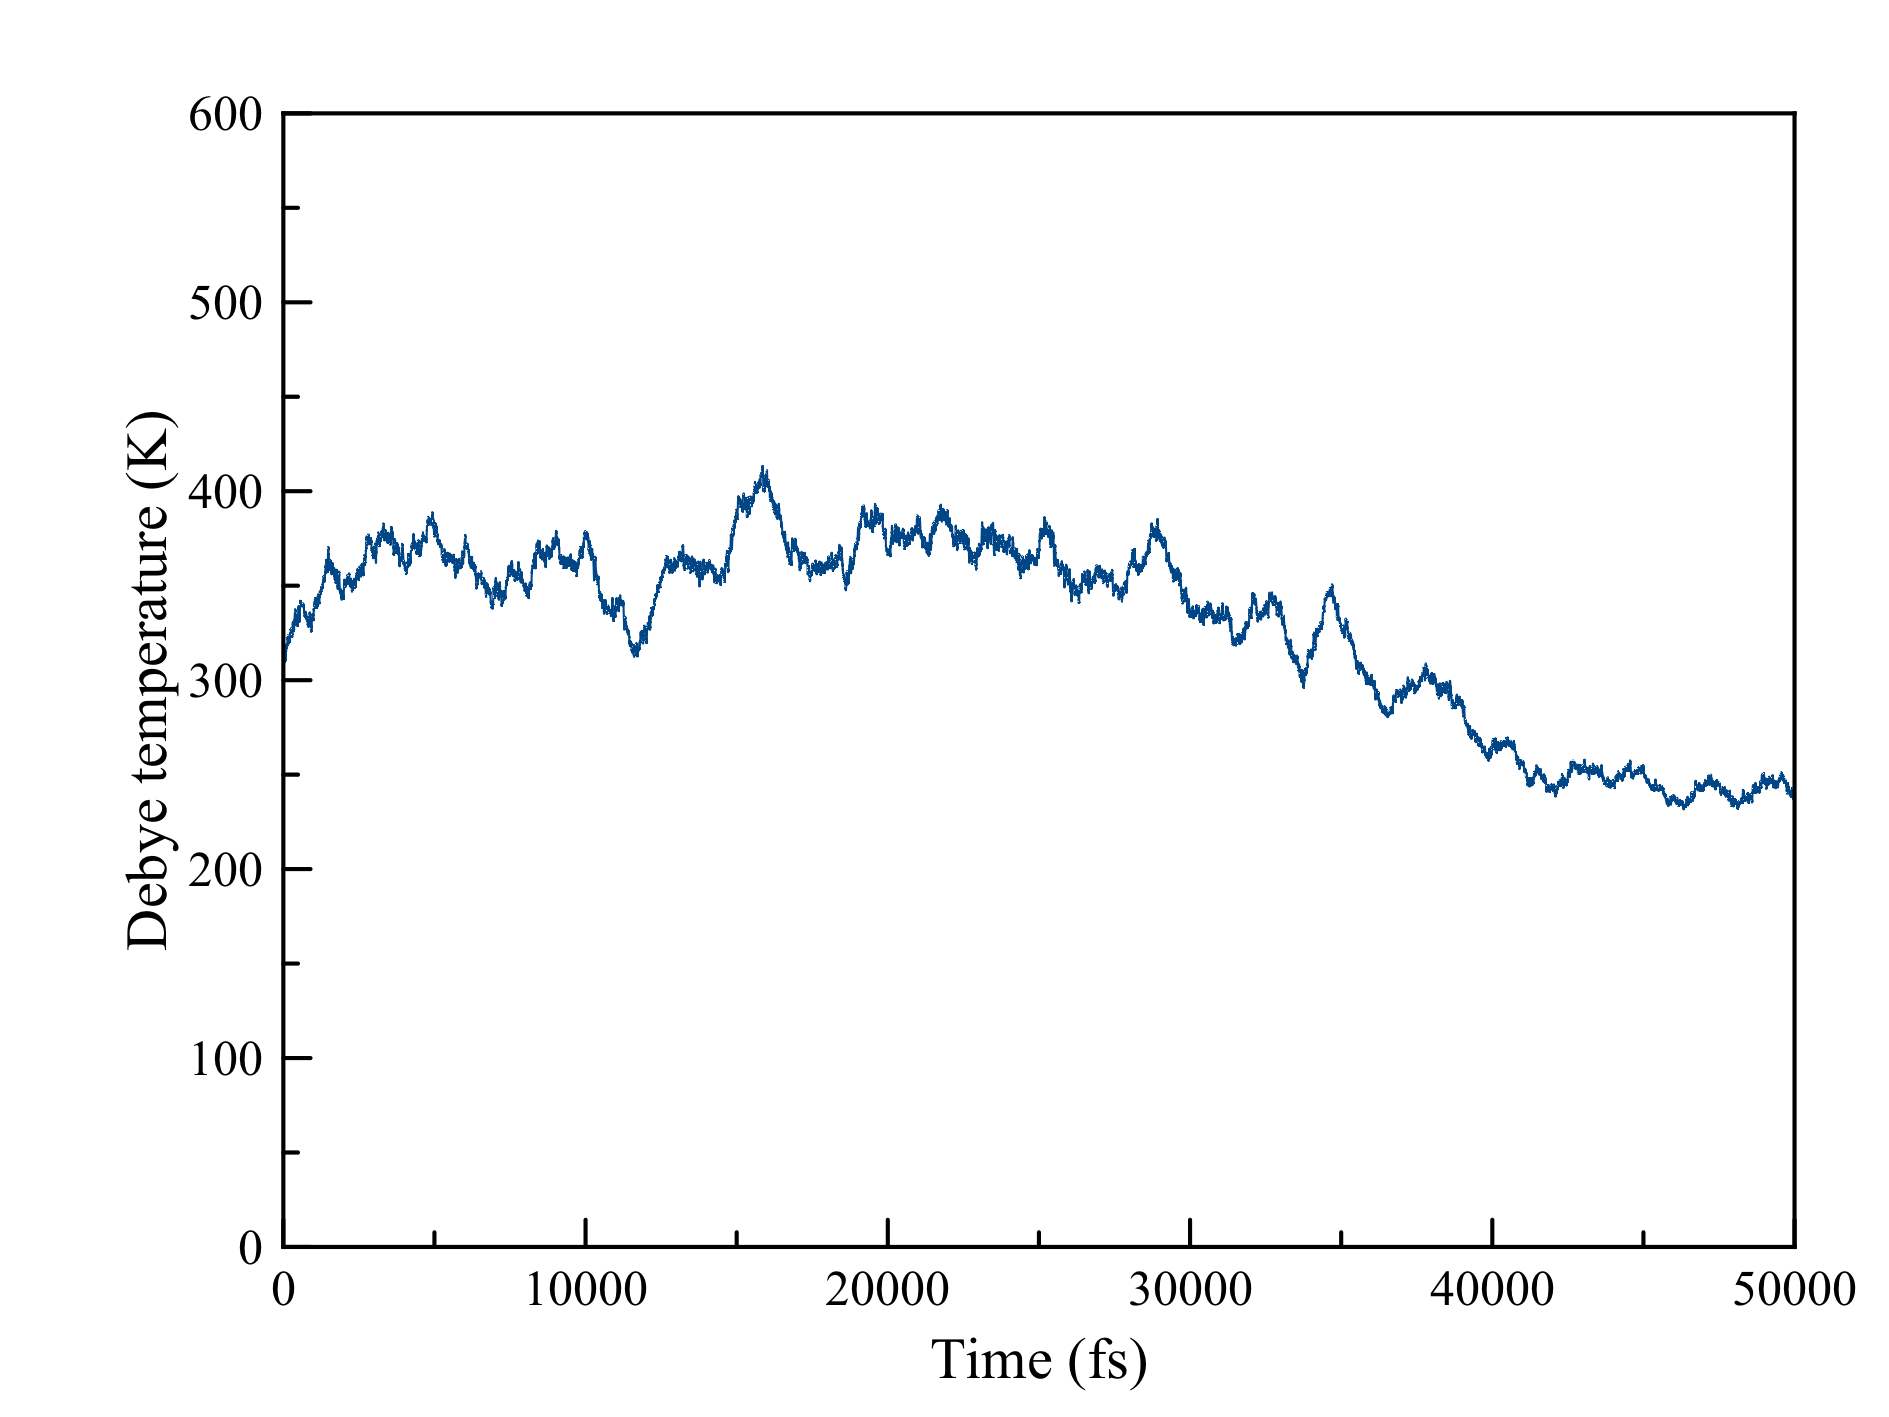
\includegraphics[width=0.7\textwidth]{debyetemp.png}
	\caption{Plotted values of the Debye temperature for bulk simulation over 50000 timesteps.}
	\label{debye}
\end{figure}

\subsubsection{Debye Temperature (surface)}
See figure \ref{debyesf}.
\begin{figure}[H]
	\centering
	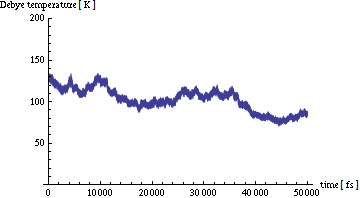
\includegraphics[width=0.7\textwidth]{debye_surface.png}
	\caption{Plotted values of the Debye temperature for surface simulation over 50000 timesteps.}
	\label{debyesf}
\end{figure}

\subsubsection{MSD (surface)}
See figure \ref{msdsf}.
\begin{figure}[H]
	\centering
	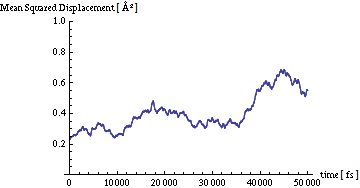
\includegraphics[width=0.7\textwidth]{msd_surface.png}
	\caption{Plotted values of the mean squared displacement for surface simulation over 50000 timesteps.}
	\label{msdsf}
\end{figure}


\subsection{Reaching equilibrium}
